%Vista lateral do robô
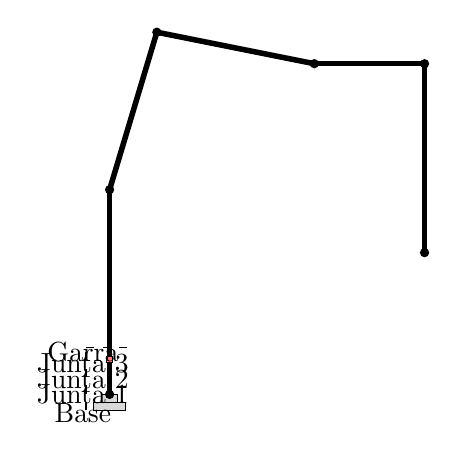
\begin{tikzpicture}[scale=0.2,
                    % Estilos
                    link/.style={line width=2pt, line cap=round},
                    junta/.style={circle, draw, fill=blue!50, line width=1pt, inner sep=2pt}]

  % Coordenadas das juntas
    \coordinate (J1) at (1,1);
    \coordinate (J2) at (1,14);
    \coordinate (J3) at (4,24);
    \coordinate (J4) at (14,22);
    \coordinate (J5) at (21,22);
    \coordinate (J6) at (21,10);

  % Base
    \draw[fill=gray!30] (0,0) rectangle (2,0.5);
    \draw[fill=gray!30] (0.5,0.5) rectangle (1.5,1);
  
  % Juntas
    \draw[junta] (J1) circle (0.2);
    \draw[junta] (J2) circle (0.2);
    \draw[junta] (J3) circle (0.2);
    \draw[junta] (J4) circle (0.2);
    \draw[junta] (J5) circle (0.2);
    \draw[junta] (J6) circle (0.2);
  
  % Braços
    \draw[link] (J1) -- (J2);
    \draw[link] (J2) -- (J3);
    \draw[link] (J3) -- (J4);
    \draw[link] (J4) -- (J5);
    \draw[link] (J5) -- (J6);
  
  % Garra
  \draw[fill=red!50] (0.8,3) rectangle (1.2,3.4);
  
  % Eixos
  \draw[dashed] (-0.5,0) -- (-0.5,4);
  \draw[dashed] (-0.5,4) -- (2.5,4);
  
  % Labels
  \node at (-0.7,-0.2) {Base};
  \node at (-0.7,1) {Junta 1};
  \node at (-0.7,2) {Junta 2};
  \node at (-0.7,3) {Junta 3};
  \node at (-0.7,3.7) {Garra};
\end{tikzpicture}